Per riuscire a calcolare l'orbita del satellite abbiamo bisogno dei sei
parametri orbitali:
\begin{itemize}
  \item eccentricità
  \item anomalia vera
  \item semi-asse maggiore
  \item RAAN (Right Ascension of the Ascending Node)
  \item argomento del perigeo
  \item inclinazione
\end{itemize}

Al fine di determinare i parametri orbitali dobbiamo prima calcolare la risposta
libera del nostro sistema. Riscriviamo l'equazione $\ref{eq:2body_acc}$ senza
considerare le forze esterne
\begin{equation}
\dot{\bf v}(t)=-\frac{\mu_0}{r^3}{\bf r(t)}, v(0)=v_0
\label{eq:free_response}
\end{equation}
La risposta libera descrive un'orbita che giace su un piano fisso, il piano
orbitale, definito dai vettori velocità e posizione. Si nota che l'accelerazione
è istante per istante opposta al vettore posizione, quindi se prendiamo in esame
il momento angolare per unità di massa {\bf h(t)}, definito come ${\bf
h(t)}={\bf r(t)}$ x ${\bf v(t)}$, la sua derivata è uguale a zero. Quindi ${\bf
h}=h{\bf e_h}$ è un vettore costante in direzione ${\bf e_h}$ (il polo dell'orbita) e
magnitudine h, che può essere preso come asse del sistema di riferimento.

Mediante il momento angolare possiamo definire il primo dei sei
parametri: il vettore eccentricità
\begin{equation}
{\bf v}(t) \times {\bf h} - \frac{\mu}{r(t)}{\bf r}(t)=\mu{\bf e}
\label{eq:eccentricity}
\end{equation}
$e=|{\bf e}|$ rappresenta  l'eccentricità dell'orbita, mentre la sua direzione
l'origine della risposta libera. La forma dell'orbita dipende dalla sua
eccentricità, esistono tre tipi di coniche in funzione del valore di $e$
\begin{itemize}
  \item ellisse per $e<1$, che diventa una circonferenza quando e=0
  \item parabola per e=1 
  \item iperbole per $e>1$
\end{itemize}
Moltiplicando scalarmente per {\bf r(t)} l'equazione \ref{eq:eccentricity} si ottiene l'equazione
della risposta libera
\begin{equation}
h^2(t)-\mu r(t)=\mu r(t)e \cos{\theta(t)}
\label{eq:free_response}
\end{equation}
$\theta$, che rappresenta l'angolo tra $r$ ed $e$, è l'anomalia vera.
Riscrivendo l'equazione \ref{eq:free_response} in funzione del raggio orbitale,
otteniamo
\begin{equation}
r(t)=\frac{p}{1+e\cos{\theta{t}}} , p=\frac{h^2}{\mu}
\end{equation}
La costante p[m] è definita semilatus rectum.

In figura \ref{fig:LVLH} è mostrata la
geometria del'orbita nel sistema di riferimento Local Vertical Local Horizontal (LVLH)
$\mathfrak{R_l}$=$\mathfrak{R}=\{C,\bar{l_1},\bar{l_2}=e_h,\bar{l_3}\}$ dove
$\bar{l_3}=\bar{e_r}=\bar{r}/r$ definisce la verticale locale, $l_1=e_{\theta}$
la orizzontale locale e $l_2=e_h$ è il polo orbitale.
\begin{figure}[htp]
\begin{center}
  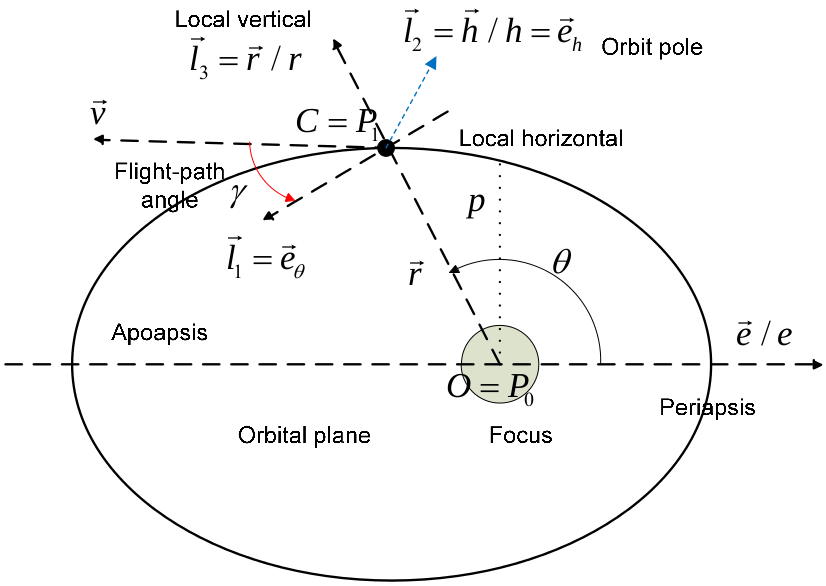
\includegraphics[width=\textwidth]{modelling/orbit_dynamics/image/LVLH.png}
  \caption{Geometria dell'orbita e sistema di riferimento LVLH}
  \label{fig:LVLH}
\end{center}
\end{figure}


Introduciamo adesso il parametro $a$, che definisce il semi-asse maggiore
dell'orbita ellittica, e l'anomalia eccentrica $E$, la quale rappresenta
l'angolo tra la linea degli absidi e la linea tra $C_0$ , centro dell’ellisse, e $Q_1$ ,
definito come la proiezione del punto $P_1$ su un cerchio ausiliario di centro
$C_0$ come illustrato in figura \ref{fig:cerchio_ausiliario}.


\begin{figure}[htp]
\begin{center}
  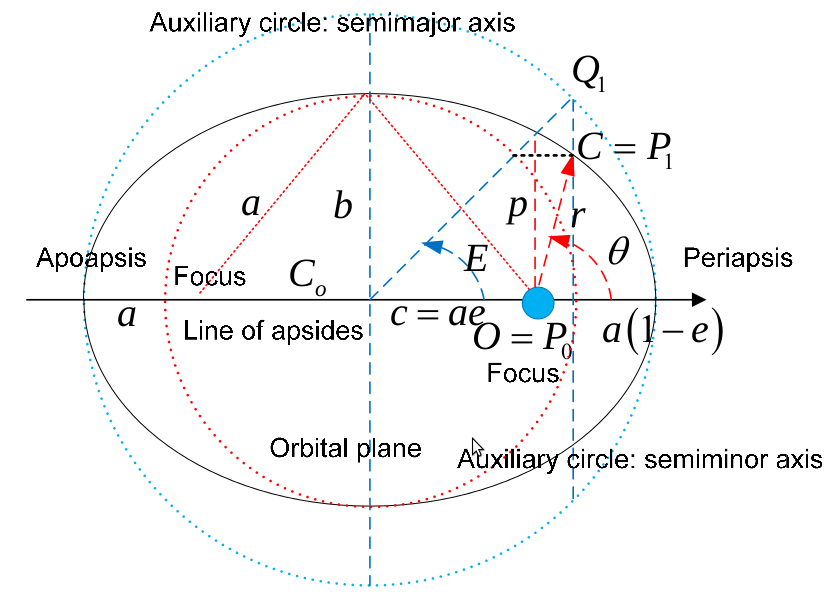
\includegraphics[width=\textwidth]{modelling/orbit_dynamics/image/cerchio_ausiliario.png}
  \caption{Geometria dell'orbita ellittica e cerchio ausiliario}
  \label{fig:cerchio_ausiliario}
\end{center}
\end{figure}

Gli ultimi parametri da definire sono: l'inclinazione tra il piano orbitale e
il piano equatoriale, il RAAN (Right Ascension of the Ascending Node),che è
l'angolo misurato sul piano equatoriale compreso tra la direzione del Punto
d'Ariete (il punto in cui il piano equatoriale incontra l'eclittica) e il Nodo
ascendente (la linea che congiunge il piano orbitale con il piano equatoriale) e
infine l'argomento del perigeo, ovvero l'angolo, sul piano orbitale, tra la
linea dei nodi e il vettore eccentricità.
Di seguito i valori inseriti nella simulazione in ambiente Matlab
\lstinputlisting[language=Matlab]{modelling/orbit_dynamics/code/orbit_parameters.m}